\subsection{Global Evaluator}

This global overview defines the baseline from which all subsequent power and precision trade-offs are derived.

\subsubsection*{Quantitative Results}
Table \ref{tab:global_benchmark} summarizes the headline results for the \texttt{ULTRA} generation of the \texttt{DetectorNX} model architecture against its \gls{cnn} counterpart.

\begin{table}[ht]
\centering
\resizebox{\textwidth}{!}{%
\begin{tabular}{|l|c|c|}
\hline
\textbf{Performance Metric} & \textbf{SNN \texttt{DetectorNX ULTRA}} & \textbf{CNN Baseline} \\
\hline
Mean IoU & 0.4658 & 0.4861 \\
\hline
Avg.\ Detections per Frame (GT) & 2.02 & 2.02 \\
Avg.\ Detections per Frame (Pred) & 1.69 & 1.75 \\
\hline
Max Confidence & 1.0000 & 0.9918 \\
Min Confidence & 0.0006 & 0.0132 \\
Mean Confidence & 0.4084 & 0.3872 \\
\hline
\end{tabular}%
}
\caption{Global Performance Benchmark results for \texttt{SNN\_MAX\_REPLICA\_SE} and 
the CNN baseline, evaluated across the full 200-sample ETraM validation set 
\parencite{Verma_2024_CVPR}. Ground truth average detections per frame is 2.02 for 
both models by definition.}
\label{tab:global_benchmark}
\end{table}

\subsubsection*{Qualitative Results}

A qualitative audit was also conducted to visualize the models' spatial reasoning across the validation subset.
Figure \ref{fig:qualitative_inference} illustrates the architectures' ability to resolve vehicle geometries in varied traffic conditions,
providing the empirical context for the subsequent critical analysis of \gls{snn} precision.

\begin{figure}[htbp]
    \centering
    \begin{subfigure}[b]{0.48\textwidth}
        \centering
        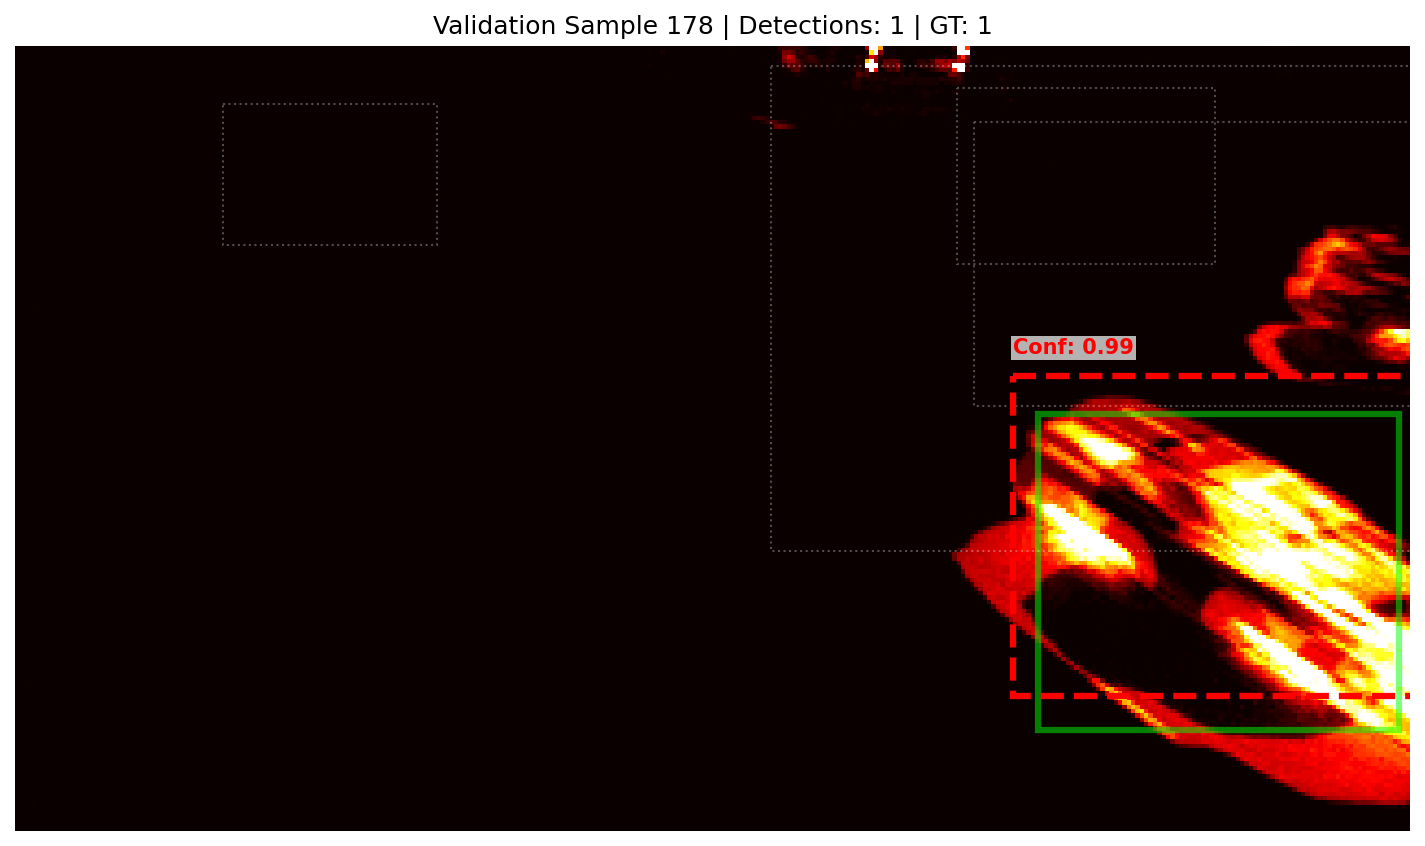
\includegraphics[width=\textwidth]{chapter_3/dnx_results/cnn_audit/audit_sample_178.png}
        \caption{CNN Baseline - Sample 1}
        \label{fig:cnn_sample1}
    \end{subfigure}
    \hfill
    \begin{subfigure}[b]{0.48\textwidth}
        \centering
        
\includegraphics[width=\textwidth]{chapter_3/dnx_results/snn_audit/audit_sample_178.png}
        \caption{SNN Ultra - Sample 1}
        \label{fig:snn_sample1}
    \end{subfigure}
    
    \vspace{1em}
    
    \begin{subfigure}[b]{0.48\textwidth}
        \centering
        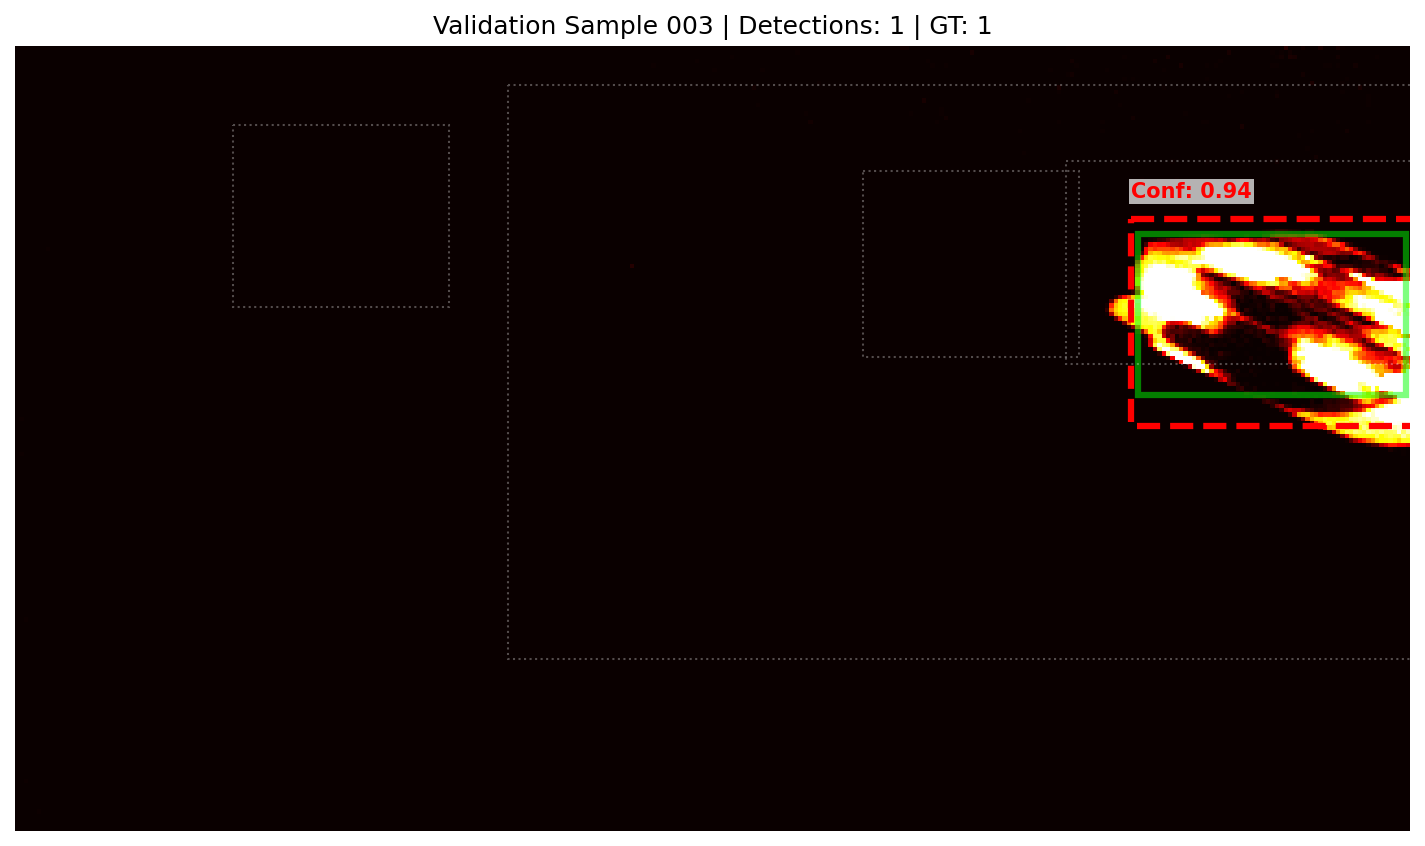
\includegraphics[width=\textwidth]{chapter_3/dnx_results/cnn_audit/audit_sample_003.png}
        \caption{CNN Baseline - Sample 2}
        \label{fig:cnn_sample2}
    \end{subfigure}
    \hfill
    \begin{subfigure}[b]{0.48\textwidth}
        \centering
        
\includegraphics[width=\textwidth]{chapter_3/dnx_results/snn_audit/audit_sample_003.png}
        \caption{SNN Ultra - Sample 2}
        \label{fig:snn_sample2}
    \end{subfigure}

    \vspace{1em}
    
    \begin{subfigure}[b]{0.48\textwidth}
        \centering
        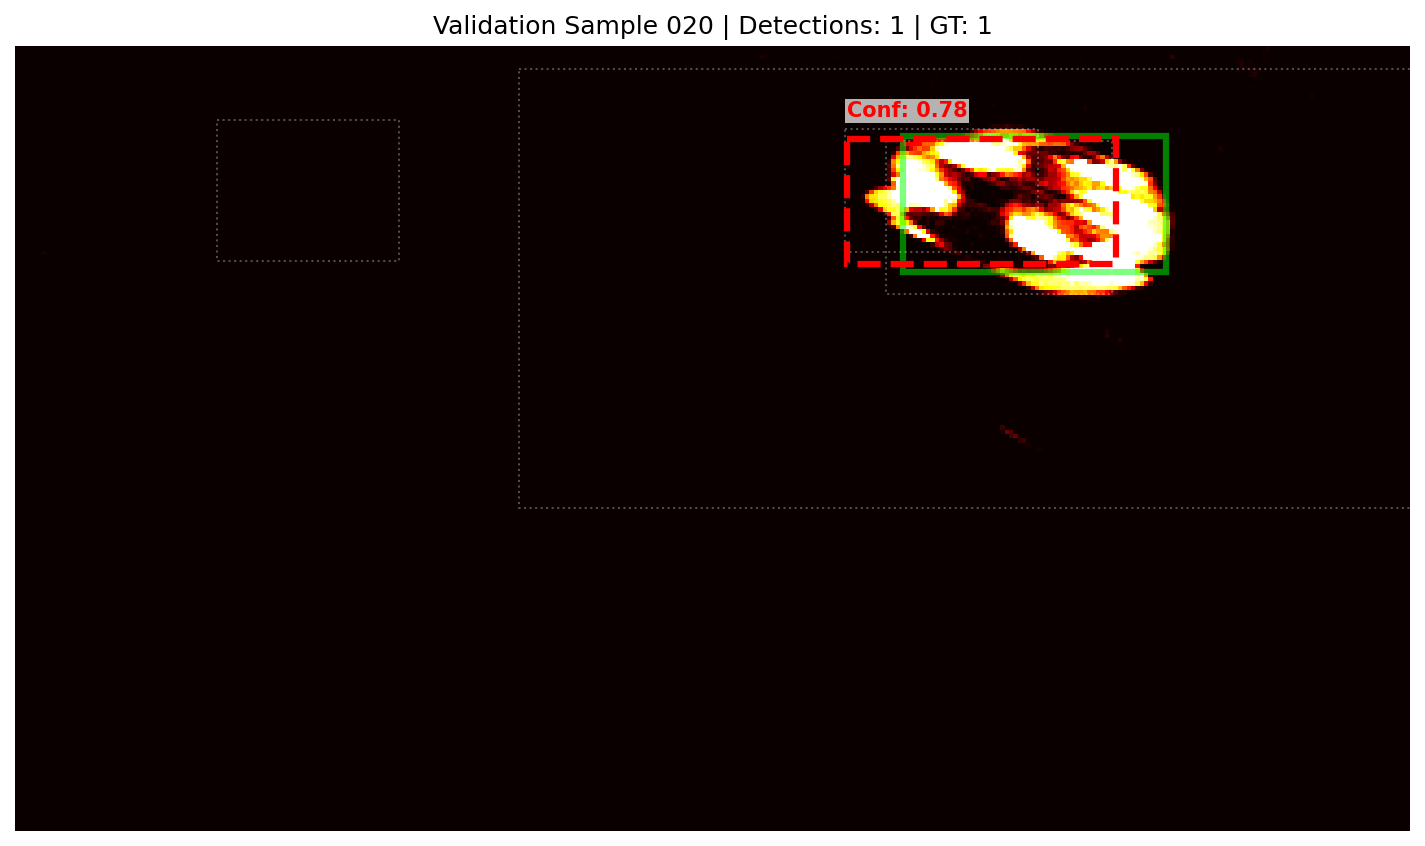
\includegraphics[width=\textwidth]{chapter_3/dnx_results/cnn_audit/audit_sample_020.png}
        \caption{CNN Baseline - Sample 3}
        \label{fig:cnn_sample3}
    \end{subfigure}
    \hfill
    \begin{subfigure}[b]{0.48\textwidth}
        \centering
        
\includegraphics[width=\textwidth]{chapter_3/dnx_results/snn_audit/audit_sample_020.png}
        \caption{SNN Ultra - Sample 3}
        \label{fig:snn_sample3}
    \end{subfigure}

    \vspace{1em}
    
    \begin{subfigure}[b]{0.48\textwidth}
        \centering
        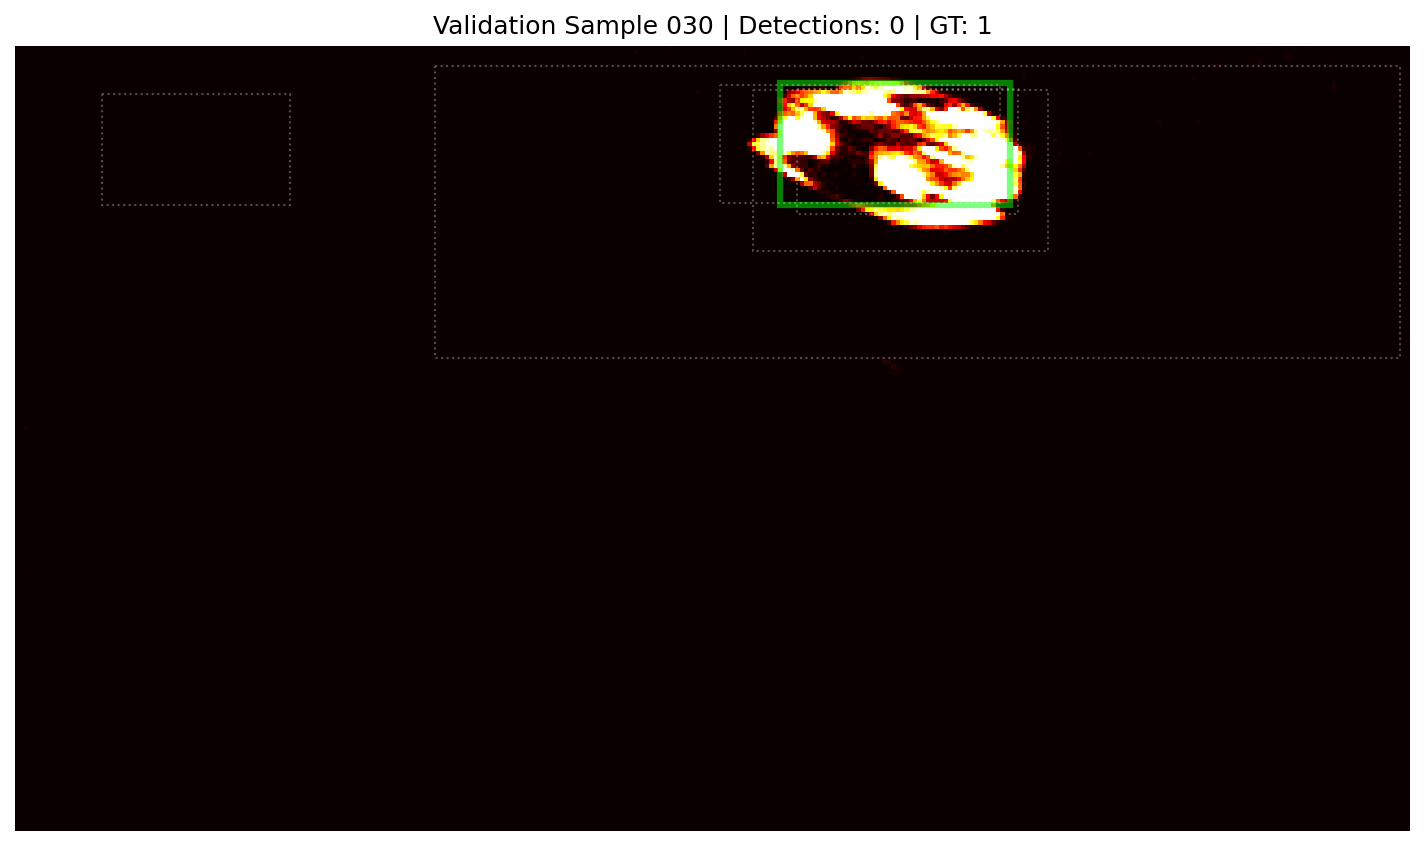
\includegraphics[width=\textwidth]{chapter_3/dnx_results/cnn_audit/audit_sample_030.png}
        \caption{CNN Baseline - Sample 4}
        \label{fig:cnn_sample4}
    \end{subfigure}
    \hfill
    \begin{subfigure}[b]{0.48\textwidth}
        \centering
        
\includegraphics[width=\textwidth]{chapter_3/dnx_results/snn_audit/audit_sample_030.png}
        \caption{SNN Ultra - Sample 4}
        \label{fig:snn_sample4}
    \end{subfigure}
    
    \caption[Qualitative Inference Audit]{Qualitative comparison of bounding box regression between the CNN baseline and SNN Ultra across representative validation samples.}
    \label{fig:qualitative_inference}
\end{figure}

\subsubsection*{Critical Analysis}